{\chapter{Ml-Agents}}
\label{sec:mlagents}
Das Unity ML-Agents Toolkit ist ein Open-Source-Projekt, in dem maschinelle Lernalgorithmen und Funktionen für die Verwendung mit der Spieleumgebung Unity implementiert und kontinuierlich weiterentwickelt werden. Die Implementierung ist in zwei Bereiche unterteilt. Für die Unity-Integration ist das Paket com.unity.ml-agents aus dem Unity Asset Store zuständig. Das eigentliche Training mit den maschinellen Lernalgorithmen findet jedoch in einer separaten Python-Umgebung statt. Für die Kommunikation zwischen den beiden Bereichen verwendet das ML-Agents Toolkit eine C\# Kommunikator-Klasse, die über gRPC-Netzwerkkommunikation mit dem Python-Prozess kommuniziert. Der Python-Prozess kommuniziert über die Python Low-Level-API, die die Kommunikation übernimmt und die Befehle an den Trainer weiterleitet.\cite{unity_mlagents_toolkit_overview}

\begin{figure}[H]
  \centering  
  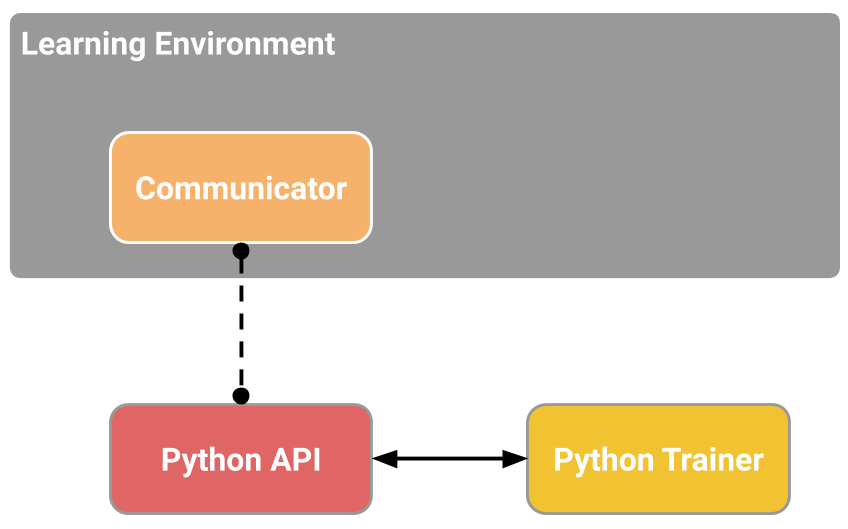
\includegraphics[scale=0.4]{img/learning_environment_basic.png}
  \caption{Unity ML-Agents Lernumgebung \protect\cite{unity_mlagents_learning_environment_basic}}
  \label{fig:learning_environment_basic}
\end{figure}

Das Unity-Paket enthält zwei Komponenten: Agenten und deren Verhalten. Die Agent-Komponente bildet die Grundlage für alle Implementierungen. Sie bietet abstrakte Funktionen für die Initialisierung, den Start einer Episode, das Erfassen des Zustands der Umgebung sowie das Ausführen von Aktionen. Durch die Implementierung dieser Funktionen können unterschiedlichste Agenten entwickelt und trainiert werden. Jeder Agent ist mit einem Verhalten verknüpft, das für jede Beobachtung des Agenten eine Aktion auswählt, die der Agent ausführt. Es gibt drei Arten, wie die Verhaltensweisen agieren können. Im Lernmodus werden die Beobachtungen des Agenten für das Training und die Auswahl einer Aktion anhand des aktuellen Modells verwendet. Der Inferenzmodus nutzt hingegen ein bereits trainiertes Modell und wertet dieses aus. Der letzte Modus eines Verhaltens ist der Heuristikmodus, bei dem festgelegte Regeln im Code entscheiden, welche Aktion ausgeführt wird, ohne die Verwendung eines trainierten Modells.\cite{unity_mlagents_toolkit_overview}

\begin{figure}[H]
  \centering  
  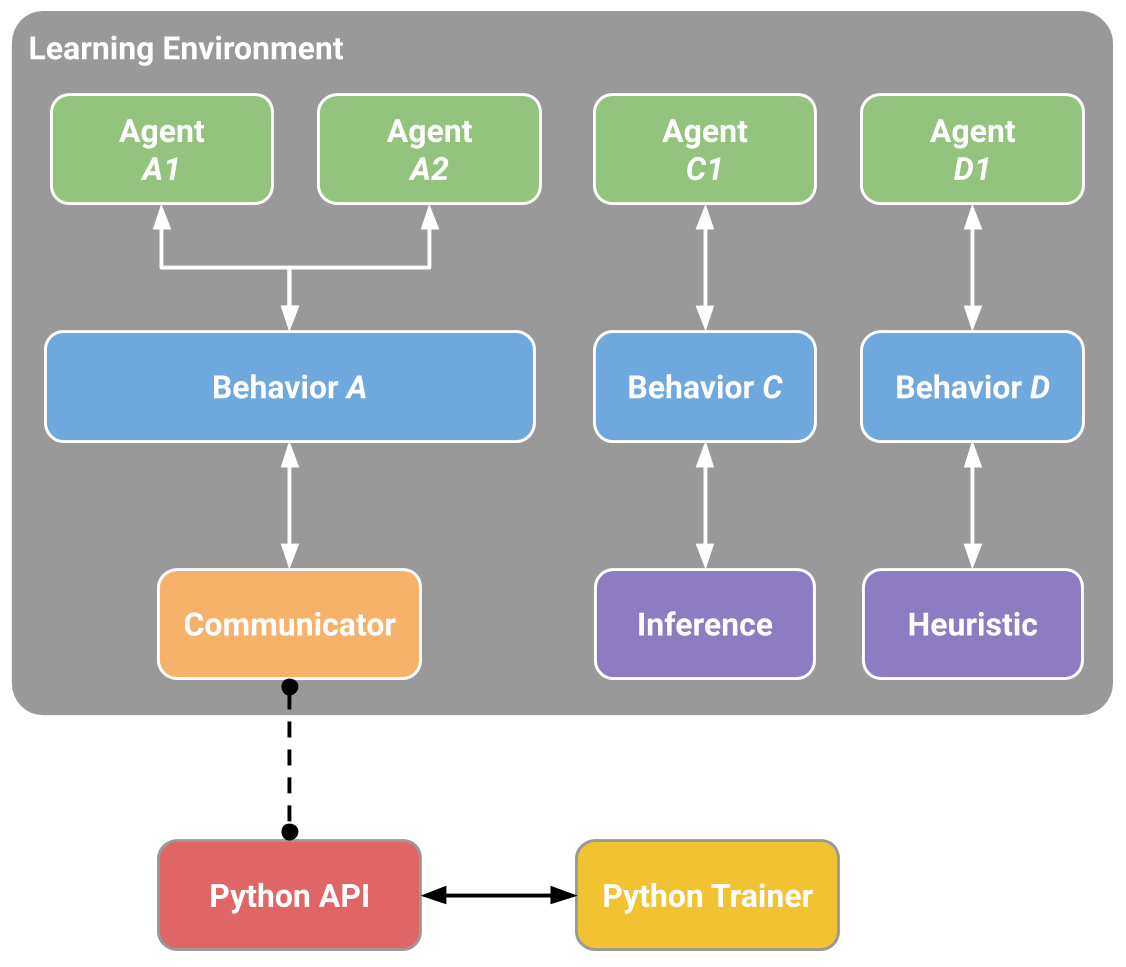
\includegraphics[scale=0.3]{img/learning_environment_example.png}
  \caption{Unity ML-Agents Lernumgebung Beispiel \protect\cite{unity_mlagents_learning_environment_example}}
  \label{fig:learning_environment_example}
\end{figure}

\section{Komponenten}

\subsection{Verhalten}
\begin{figure}[H]
  \centering  
  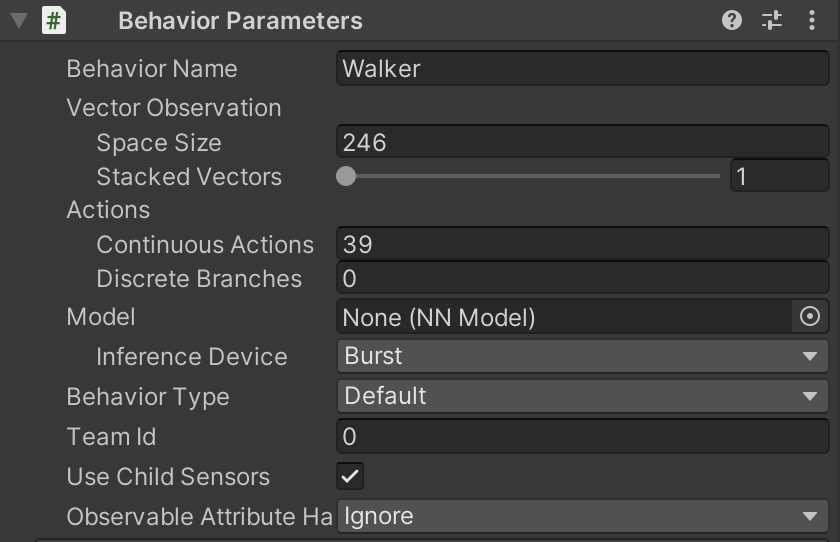
\includegraphics[scale=0.5]{img/verhalten_komponente.png}
  \caption{Unity ML-Agents Verhalten Komponente}
  \label{fig:verhalten_komponente}
\end{figure}

\begin{center}
{\rowcolors{2}{lightgray}{gray!50!lightgray!50}
\begin{tabular}{ |p{4cm}|p{8cm}| }
\hline
Konfigurationsfeld& Beschreibung \\
\hline
Behaviour Name & Name des Verhaltens / wird in Trainer Konfiguration referenziert \\
Space Size & Anzahl an Beobachtungen / Inputknoten für NN \\
Continuous Actions & Anzahl an Aktionen / Outputknoten von NN \\
Model & Referenz auf bereits trainiertes Modell zur Verwendung in Inferenz \\
Behaviour Type & Lernmodus Default = Lernen, Heuristic, Inferenz \\
\hline
\end{tabular}}
\end{center}

\subsection{Entscheidung}
\begin{figure}[H]
  \centering  
  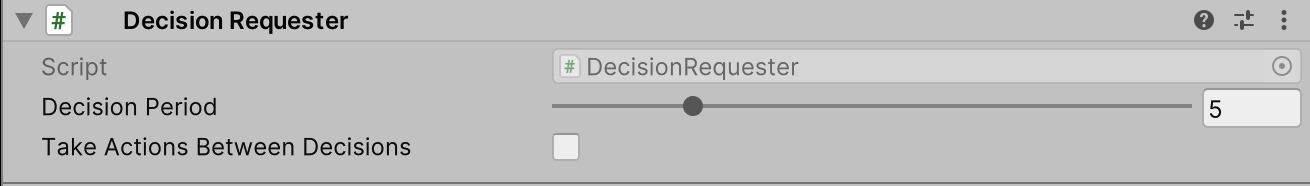
\includegraphics[scale=0.5]{img/entscheidung_anfragen_komponente.png}
  \caption{Unity ML-Agents Entscheidung Anfragen Komponente}
  \label{fig:entscheidung_anfragen_komponente}
\end{figure}

\begin{center}
{\rowcolors{2}{lightgray}{gray!50!lightgray!50}
\begin{tabular}{ |p{4cm}|p{8cm}| }
\hline
Konfigurationsfeld& Beschreibung \\
\hline
Decision Period & Anzahl an Physikupdates bis zur nächsten Entscheidung \\
Take Actions Between Decisions &  Kontrollkasten ob Agent Aktionen zwischen Entscheidungen ausführen soll \\
\hline
\end{tabular}}
\end{center}


\subsection{Agent Abstrakte Funktionen}
\begin{lstlisting}
public class TestAgent : Agent
{
    //Wird beim ersten initialisieren des Agenten ausgeführt
    public override void Initialize()
    {
        //Stellt Umgebungsparameter aus Trainer Konfiguration oder aktueller Lektion bereit
        envParams = Academy.Instance.EnvironmentParameters;
        //Schreibt Daten zur Visualisierung und Auswertung in Dateien welche von Tensorboard ausgelesen und dargestellt werden
        statsRecorder = Academy.Instance.StatsRecorder;
    }

    //Wird beim Start jeder Trainingsepisode ausgeführt
    public override void OnEpisodeBegin()
    {
    
    }

    //Wird bei jeder angefragten Entscheidung ausgeführt
    public override void CollectObservations(VectorSensor sensor)
    {
        //Hier wird der Beobachtungssensor mit Daten befüllt
        sensor.AddObservation(floatObservation);
    }

    //Wird bei jeder Entscheidung ausgeführt
    public override void OnActionReceived(ActionBuffers actionBuffers)
    {
        //Hier werden die Float Werte vom NN in Aktionen umgewandelt
        var continuousActions = actionBuffers.ContinuousActions;
        float action = continuousActions[0]
    }

    public virtual void FixedUpdate()
    {
        //Mit der AddReward Funktion können überall Belohnungen implementiert werden
        AddReward(floatReward);
    }
}

\end{lstlisting}

TODO:
Trainer Konfigurationsdatei
